\documentclass[a4paper]{article}
\usepackage[T1]{fontenc}
\usepackage{graphicx}
\usepackage{algorithm}
\usepackage{algorithmic}
\usepackage[utf8]{inputenc}
\usepackage{lmodern}
\usepackage{amsmath,amssymb}
\usepackage{geometry}

\geometry{
  a4paper,
  left=25mm,
  right=25mm,
  top=25mm,
  bottom=25mm
}

\title{WSI Labolatorium 2}
\author{Jonatan Kasperczak 341208}
\date{March 2025}

\begin{document}
\maketitle
\section{Wprowadzenie}
Celem projektu jest porównanie efektywności dwóch metod optymalizacji:
\begin{itemize}
  \item algorytmu \textbf{ewolucyjnego}, opartego na losowej modyfikacji i selekcji populacji kandydatów,
  \item klasycznego \textbf{algorytmu gradientu prostego}, korzystającego z pochodnej funkcji celu.
\end{itemize}

Obie metody przetestowano na dwóch funkcjach testowych z zestawu \textbf{CEC2017}:
\begin{enumerate}
  \item \textbf{F3} – Rotated High Conditioned Elliptic Function
  \item \textbf{F19} – Composition Function złożona z funkcji Rosenbrocka, Ackley i Weierstrass
\end{enumerate}

Funkcje te są znane z trudności optymalizacji, a ich minimum globalne wynosi $f(x^*) = 0$.  
W obu przypadkach zastosowano przestrzeń \(\mathbb{R}^{10}\) i punkt początkowy losowany z rozkładu jednostajnego.  
Dla algorytmu ewolucyjnego przeprowadzono uśrednione testy, natomiast metoda gradientowa była oceniana osobno.  
Celem było zaobserwowanie zbieżności, stabilności oraz jakości uzyskanych wyników.

\section{Algorytm ewolucyjny}

Algorytm ewolucyjny działa na populacji $P$ wektorów rzeczywistych $x \in \mathbb{R}^n$, które są kandydatami do optymalnego rozwiązania.  
W każdej iteracji obliczana jest wartość funkcji celu dla każdego osobnika, a następnie generowana jest nowa populacja na podstawie losowo wybranych rodziców oraz mutacji Gaussowskiej.

Zastosowano elitaryzm: najlepszy osobnik z dotychczasowych iteracji zostaje przeniesiony bez zmian do nowej populacji.  
Mutacja osłabia się w trakcie działania algorytmu (\emph{mutation strength} maleje liniowo).  
Obliczenia są przerywane, jeśli przez 300 kolejnych iteracji nie uda się poprawić najlepszego wyniku.

\subsection{Parametry algorytmu}
\begin{itemize}
  \item \textbf{pop\_size} – liczba osobników w populacji (np.~500),
  \item \textbf{max\_iter} – maksymalna liczba iteracji (np.~3000),
  \item \textbf{mutation\_prob} – prawdopodobieństwo mutacji (np.~0.8),
  \item \textbf{mutation\_strength} – siła mutacji początkowej (np.~6.0),
  \item \textbf{tol} – tolerancja (nieaktywna w tej wersji),
  \item \textbf{max\_improve\_c} – liczba iteracji bez poprawy po której następuje przerwanie działania (ustalona na 300).
\end{itemize}

\begin{algorithm}[H]
\caption{Algorytm ewolucyjny z elitaryzmem i zanikającą mutacją}
\label{alg:evolutionary}
\begin{algorithmic}[1]

\REQUIRE
  Funkcja celu \(f\); liczba osobników \(N\); maksymalna liczba iteracji \(\text{maxIter}\); parametry mutacji.

\STATE \( P \leftarrow \text{populacja losowa z rozkładu } [-100, 100]^n \)
\STATE \( \text{best} \leftarrow \arg\min_{x \in P} f(x) \)
\STATE \( \text{bestFit} \leftarrow f(\text{best}) \)
\STATE \( \text{counter} \leftarrow 0 \)

\FOR{\(i = 1 \text{ to } \text{maxIter}\)}

  \STATE Oblicz wartości \(f(x)\) dla wszystkich \(x \in P\)
  \STATE \( x_{\text{best}} \leftarrow \arg\min_{x \in P} f(x) \)

  \IF{\(f(x_{\text{best}}) < \text{bestFit}\)}
    \STATE \( \text{best} \leftarrow x_{\text{best}},\quad \text{bestFit} \leftarrow f(x_{\text{best}}) \)
    \STATE \( \text{counter} \leftarrow 0 \)
  \ELSE
    \STATE \( \text{counter} \leftarrow \text{counter} + 1 \)
  \ENDIF

  \IF{\( \text{counter} = 300 \)} \STATE \textbf{break} \ENDIF

  \STATE Wylicz siłę mutacji: \( \sigma = \text{mutationStrength} \cdot (1 - \tfrac{i}{\text{maxIter}}) \)

  \STATE \( P_{\text{new}} \leftarrow [\;] \)
  \FOR{\(j = 1 \text{ to } N-1\)}
    \STATE Wybierz losowego osobnika \( x \in P \)
    \IF{losowa liczba < mutation\_prob}
      \STATE Dodaj mutację \(x \leftarrow x + \mathcal{N}(0, \sigma^2)\)
    \ENDIF
    \STATE Dodaj \(x\) do \(P_{\text{new}}\)
  \ENDFOR

  \STATE Dodaj najlepszy osobnik do \(P_{\text{new}}\)
  \STATE \( P \leftarrow P_{\text{new}} \)

\ENDFOR
\STATE \textbf{return} najlepszy osobnik i jego wartość

\end{algorithmic}
\end{algorithm}

\section{Testowanie algorytmu ewolucyjnego}

W celu zbadania zbieżności algorytmu ewolucyjnego przeprowadzono eksperymenty na funkcjach F3 oraz F19 z zestawu CEC2017.  
Każda funkcja była optymalizowana 10-krotnie dla wymiarowości \(n=10\), a wyniki uśredniane.  


\begin{table}[H]
\centering
\begin{tabular}{|c|c|}
\hline
\textbf{Funkcja} & \textbf{Średnia liczba iteracji} \\\hline
F3 & 1117.4 \\\hline
F19 & 587.6 \\\hline
\end{tabular}
\caption{Średnia liczba iteracji do zatrzymania dla 10 uruchomień}
\end{table}


\begin{table}[H]
\centering
\begin{tabular}{|c|c|c|}
\hline
\textbf{Uruchomienie} & \textbf{F3} & \textbf{F19} \\\hline
Run 1 & 538.60 & 4636.10 \\\hline
Run 2 & 374.10 & 2738.60 \\\hline
Run 3 & 408.92 & 2283.40 \\\hline
Run 4 & 423.75 & 2908.80 \\\hline
Run 5 & 513.71 & 15420.00 \\\hline
Run 6 & 413.88 & 3643.80 \\\hline
Run 7 & 806.56 & 2736.30 \\\hline
Run 8 & 342.33 & 1958.80 \\\hline
Run 9 & 385.23 & 2366.60 \\\hline
Run 10 & 674.08 & 6150.70 \\\hline
\textbf{Średnia} & \textbf{488.32} & \textbf{4304.27} \\\hline
\end{tabular}
\caption{Końcowe wartości \(f(x)\) po działaniu algorytmu ewolucyjnego (10 uruchomień)}
\end{table}

\subsection{Średnia zbieżność dla F3 i F19}

\begin{figure}[H]
    \centering
    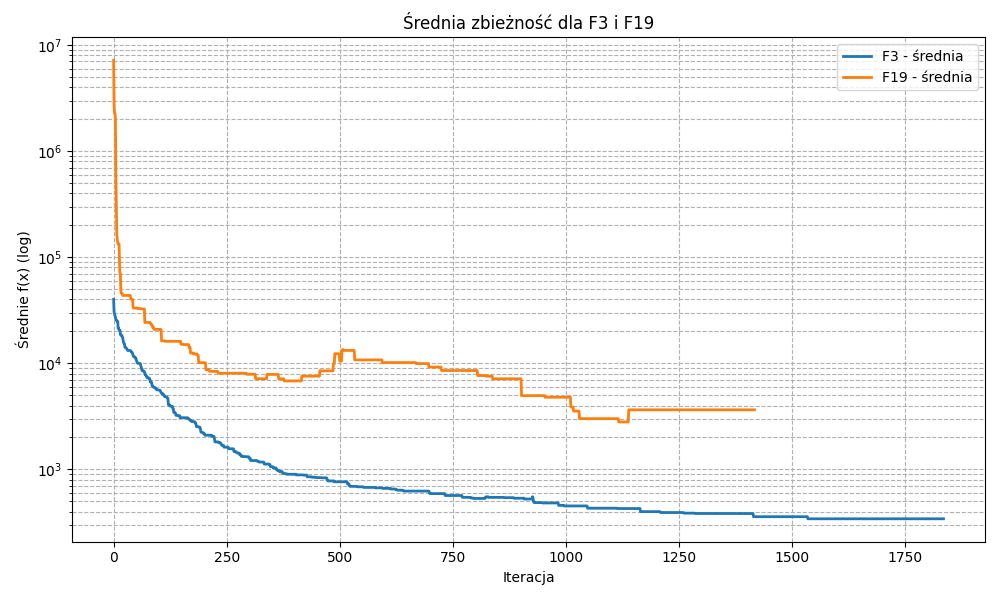
\includegraphics[width=0.6\linewidth]{avg_convergence_plot.png}
    \caption{Średnia wartość \(f(x)\) w skali logarytmicznej (10 uruchomień algorytmu ewolucyjnego)}
    \label{fig:avg_convergence}
\end{figure}

Na rysunku~\ref{fig:avg_convergence} przedstawiono uśrednioną wartość \(f(x)\) w kolejnych iteracjach.  
Widać wyraźnie, że dla funkcji F3 zbieżność jest szybsza i stabilniejsza – już po kilkuset iteracjach następuje spłaszczenie krzywej.  
Dla F19 wartości są początkowo wyższe i opadają wolniej, a moment stabilizacji jest mniej wyraźny.  
Oznacza to większą trudność w eksploracji przestrzeni i potrzebę większej liczby prób losowych.

\subsection{Zbieżność funkcji F3 – wszystkie uruchomienia}

\begin{figure}[H]
    \centering
    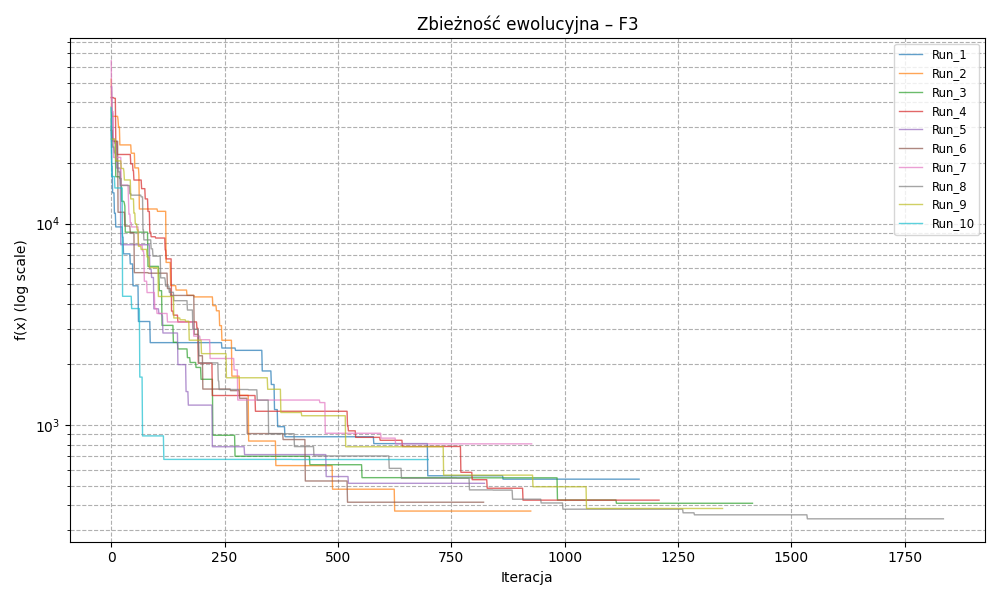
\includegraphics[width=0.6\linewidth]{F3_log_plot.png}
    \caption{Zbieżność funkcji F3 (10 uruchomień, skala logarytmiczna)}
    \label{fig:f3log}
\end{figure}

Na wykresie~\ref{fig:f3log} widzimy, że przebiegi 10 uruchomień są bardzo zbliżone – każda krzywa opada szybko w kierunku minimum, co świadczy o niskiej wariancji rozwiązania.  
Algorytm ewolucyjny w tym przypadku działa stabilnie i powtarzalnie.

\subsection{Zbieżność funkcji F19 – wszystkie uruchomienia}

\begin{figure}[H]
    \centering
    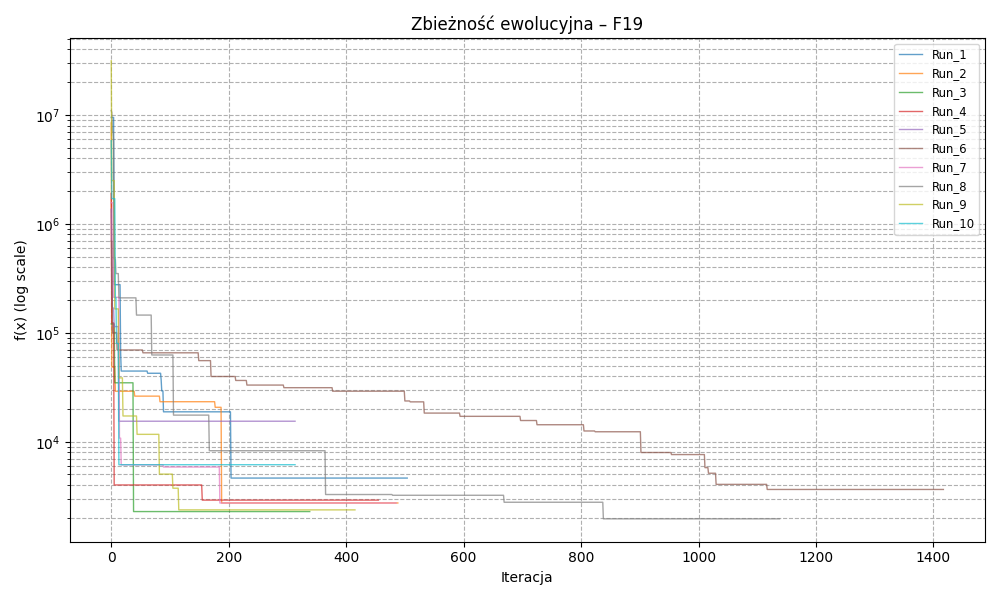
\includegraphics[width=0.6\linewidth]{F19_log_plot.png}
    \caption{Zbieżność funkcji F19 (10 uruchomień, skala logarytmiczna)}
    \label{fig:f19log}
\end{figure}

Rysunek~\ref{fig:f19log} pokazuje znacznie większe rozproszenie wartości końcowych.  
Część uruchomień zakończyła się z bardzo niskim \(f(x)\), inne „utknęły” wyżej – co potwierdza obecność licznych minimów lokalnych i trudność funkcji F19.  
Jest to typowe dla funkcji kompozycyjnych, w których różne składniki (np. Weierstrass) generują wielomodalne krajobrazy.


\section{Porównanie z metodą gradientu prostego}

W celu pełnego zrozumienia skuteczności zaprojektowanego algorytmu ewolucyjnego, przeprowadzono także analogiczne testy z wykorzystaniem metody gradientu prostego.  

\subsection{Funkcja F3 – Gradient prosty}

Funkcja F3 to \emph{Rotated High Conditioned Elliptic Function}, czyli eliptyczna funkcja o bardzo dużej kondycji (kondycja macierzy hessjan to rzędu $10^6$).  
Gradient tej funkcji w różnych kierunkach ma dramatycznie różne skale, co sprawia, że stały krok \(\alpha\) nie pozwala na skuteczną aktualizację współrzędnych jednocześnie.

Wszystkie uruchomienia gradientu zakończyły się bez sukcesu, z bardzo dużymi końcowymi wartościami funkcji celu (rzędu \(10^{10}\)), pomimo pełnego wykonania 20000 iteracji.  
Wektor rozwiązania nie zbiegał do minimum, lecz często „wahał się” w rejonach dalekich od optimum globalnego.

\subsection{Funkcja F19 – Gradient prosty}

Funkcja F19 jest jedną z najbardziej złożonych funkcji benchmarku CEC2017.  
Stanowi kompozycję funkcji Rosenbrocka, Ackley i Weierstrassa, czyli łączy trudności wynikające z:
\begin{itemize}
  \item licznych minimów lokalnych,
  \item bardzo płaskich fragmentów przestrzeni,
  \item silnie niestabilnych i oscylujących gradientów.
\end{itemize}

Dla funkcji F19 jedynie przy ekstremalnie małych wartościach kroku uczenia (\(\alpha = 10^{-5}\)) udawało się zbiec do względnie sensownych wyników (np.~\(f(x) \approx 500\)), ale nawet w takich przypadkach nie był spełniony warunek stopu i algorytm wykonywał pełne 20000 iteracji.

\section{Wykresy dla metody gradientu prostego}

\begin{figure}[H]
    \centering
    \begin{minipage}{0.48\linewidth}
        \centering
        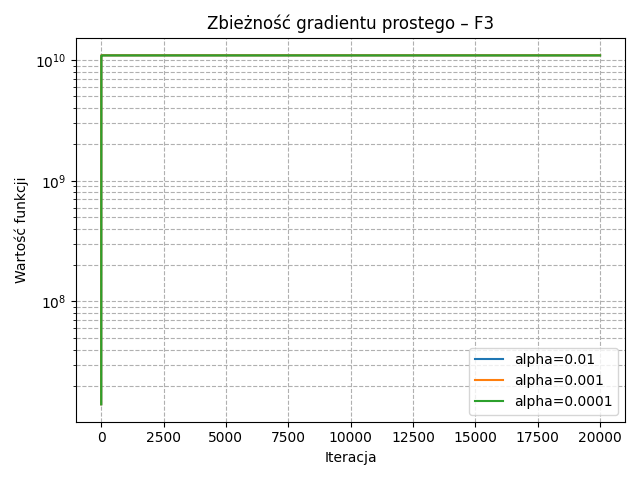
\includegraphics[width=\linewidth]{F3_gradient_plot.png}
        \caption{Gradient – przebieg wartości \(f(x)\) dla F3}
        \label{fig:f3grad}
    \end{minipage}
    \hfill
    \begin{minipage}{0.48\linewidth}
        \centering
        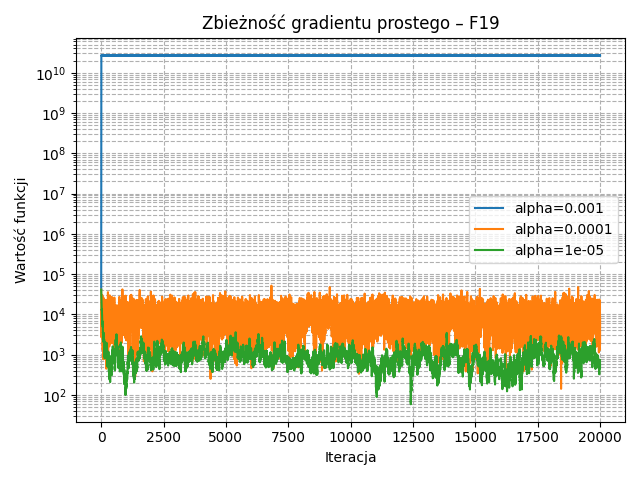
\includegraphics[width=\linewidth]{F19_gradient_plot.png}
        \caption{Gradient – przebieg wartości \(f(x)\) dla F19}
        \label{fig:f19grad}
    \end{minipage}
\end{figure}


\subsection{Wnioski wynikające z porównania metod}

\begin{itemize}
  \item Metoda gradientu prostego z jednym, stałym krokiem \(\alpha\) okazuje się nieefektywna na złożonych funkcjach testowych z benchmarku CEC2017.
  \item Dla funkcji F3 różnice w skali gradientu pomiędzy współrzędnymi powodują, że krok dobrany odpowiednio dla jednej współrzędnej jest zbyt duży lub zbyt mały dla innych.
  \item Dla funkcji F19 obecność oscylujących składników i wielu minimów lokalnych prowadzi do bardzo niestabilnej zbieżności.
  \item Algorytm ewolucyjny, mimo swojej prostoty i braku wykorzystania pochodnej, poradził sobie zdecydowanie lepiej — co jest szczególnie widoczne w przypadku F19, gdzie wartości \(f(x)\) po 1000 iteracjach były nawet 10-krotnie niższe niż w metodzie gradientowej po 20000 iteracjach.
  \item Dla trudnych funkcji nieliniowych o niegładkich lub nieciągłych gradientach algorytmy populacyjne okazują się bardziej odporne i skuteczniejsze.
\end{itemize}

\section{Podsumowanie}
Na podstawie przeprowadzonych eksperymentów można sformułować następujące wnioski:

\begin{itemize}
  \item \textbf{Algorytm ewolucyjny} poradził sobie bardzo dobrze z optymalizacją funkcji F3 i F19 – szczególnie przy zastosowaniu elitaryzmu oraz osłabiającej się mutacji.
  \item Dla F3 wyniki były stabilne i powtarzalne, z niską wariancją i szybką zbieżnością.  
        Średnia liczba iteracji do zatrzymania to około 1100.
  \item Dla F19 zbieżność była trudniejsza – z powodu lokalnych minimów i bardziej złożonego krajobrazu funkcji.  
        Algorytm jednak osiągał dobre wyniki w mniej niż 600 iteracjach średnio.
  \item \textbf{Metoda gradientu prostego} nie była w stanie skutecznie zoptymalizować żadnej z funkcji przy zastosowaniu stałego kroku.  
        Dla F3 – rozbieżność przez różną skalę gradientu, dla F19 – niestabilność i utknięcie w minimach lokalnych.
  \item Optymalizacja funkcji o złej kondycji lub złożonej strukturze wymaga metod nieliniowych i adaptacyjnych.  
        Algorytmy populacyjne są tu znacznie bardziej odporne i efektywne, nawet bez informacji o pochodnej.
\end{itemize}

Projekt potwierdził zasadność stosowania algorytmów ewolucyjnych w zadaniach, gdzie klasyczne metody gradientowe zawodzą. W zastosowaniach praktycznych, gdy funkcje są trudne do analitycznego opisu lub mają nieregularne krajobrazy optymalizacji, metody populacyjne stanowią bardziej uniwersalne i odporne podejście.

\end{document}